%	https://tikz.net/desargues/
\documentclass[tikz,border=10pt]{standalone} 
\usetikzlibrary{calc,intersections} 
\begin{document} 
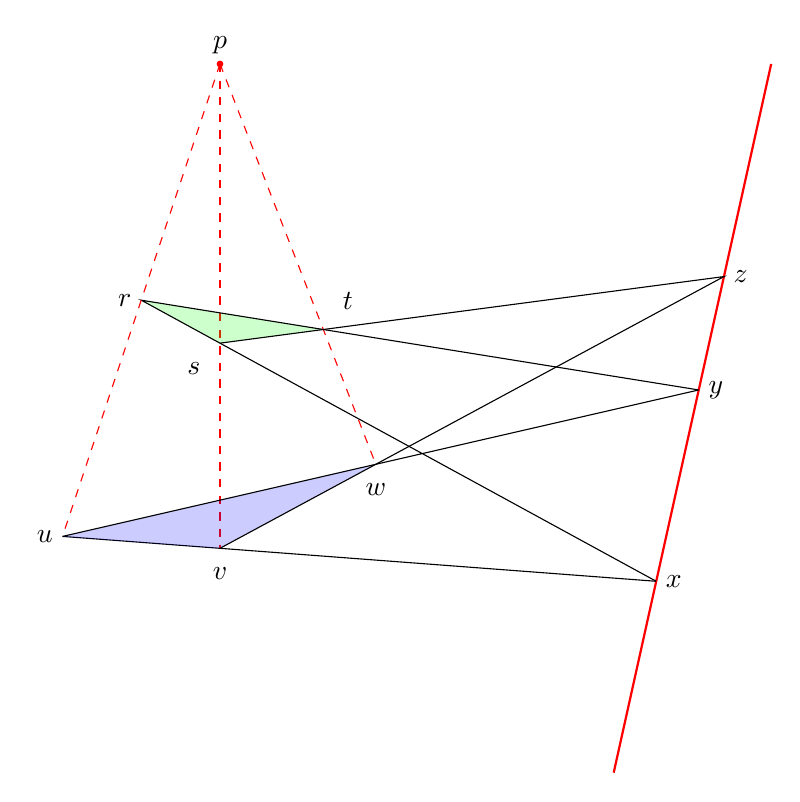
\begin{tikzpicture}
  \coordinate [label=above:$p$] (p) at (2,9); 
  \coordinate [label=left:$u$] (u) at (0,3); 
  \coordinate [label=left:$r$] (r) at ($(p)!0.5!(u)$); 
  % modification of numbers gives you modified illustrations
  \coordinate (q) at (2,2); 
  \coordinate (l) at (7,0); 
  \coordinate (m) at (9,9); 
  \coordinate [label=right:$x$] (x) at ($(l)!0.27!(m)$); 
  \coordinate [label=right:$y$] (y) at ($(l)!0.54!(m)$); 
  \coordinate [label=right:$z$] (z) at ($(l)!0.7!(m)$); 
  \draw [color=red,thick] (l) -- (m); 
  \path [name path = pq] (p) -- (q); 
  \draw [name path = ux] (u) -- (x); 
  \path [name intersections={of = pq and ux,by = v}]; 
  \node [label=below:$v$] at (v) {}; 
  \draw [color=red,dashed] (p) -- (v); 
  \path [name path = uy] (u) -- (y); 
  \path [name path = vz] (v) -- (z); 
  \path [name intersections={of = uy and vz,by = w}]; 
  \node [label=below:$w$] at (w) {}; 
  \draw [color=red,dashed,name path=pw] (p) -- (w); 
  \path [name path = rx] (r) -- (x); 
  \path [name path = ry] (r) -- (y); 
  \path [name intersections={of = pq and rx,by = s}]; 
  \node [label=below left:$s$] at (s) {}; 
  \path [name intersections={of = pw and ry,by = t}]; 
  \node [label=above right:$t$] at (t) {}; 
  \fill [color=green,opacity=0.2] (r) -- (s) -- (t) -- (r); 
  \fill [color=blue,opacity=0.2] (u) -- (v) -- (w) -- (u); 
  \draw (x) -- (r) -- (y) (u) -- (y); 
  \filldraw [fill=red,draw=red] (p) circle(1pt); 
  \draw (s) -- (z) -- (v); 
  \draw [color=red,dashed] (p) -- (u); 
\end{tikzpicture} 
\end{document}